\subsubsection{Humain}
\begin{samepage}
	\begin{flushright}
		\begin{tabular}{ l l }
			\textbf{Type} 			& Humanoïde \\
		   	\textbf{Planète} 		& Terre \\
		   	\textbf{Language} 		& Basic \\
		   	\textbf{Orientation} 	& Neutre \\
		\end{tabular}
	\end{flushright}

	\vspace{-6\baselineskip}
	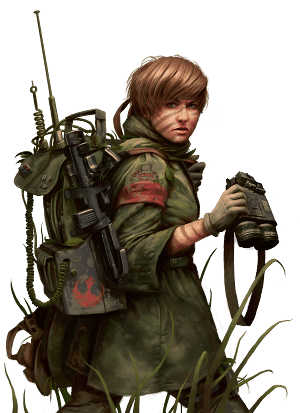
\includegraphics[width=5cm]{img/races/humain.png} 
\end{samepage}

Cette race comprend aussi bien les humains au sens strict (qu’ils soient originaires de Coruscant, de Correlia, de Kuat, de Naboo...) que les humanoïdes dont les caractéristiques physiques, intellectuelles, sociales et culturelles sont suffisamment proches de celles des humains pour qu’il soit possible de les assimiler en termes de jeu. Cela inclut par exemple les iridoniens (zabraks) et les dévaroniens.

\begin{description}[align=left]
\item [Adaptabilité] 	%CAP +2
	Les humains sont une race pleine de ressources, ils s'adaptent rapidement à toutes sorte de difficultés ou environnements.\\
	\emph{Compétence à d6}
\end{description}